As stated in the Introduction, the goal of this thesis is to use a neural network to identify the droplets in the captured image data. The problem lies in the domain of \emph{segmantic pixel level image segmentation} and the employed network is a kind of \emph{(Deep-)Convolutional Neural Network} (DCNN). In the following section, a brief overview of the basics of neural networks, how they work in general and how they can be adapted to a certain task is given. 

\subsection{Basics and buidling blocks of neural networks}
\label{sec:building_blocks}

The idea of artificial neural networks came long before the capability to employ them as a tool and stems from research in trying to model how biological neurons function. Biological nerve cells receive signals from several other neurons and send a signal on their own based on the strength of their inputs. Translating this behaviour to a mathematical model brings us to the \emph{single layer perceptron}.

\paragraph*{Perceptron}

\begin{figure}[htbp]
    \makebox[\textwidth][c]{
    \tikzset{basic/.style={draw,fill=blue!20,text width=1em,text badly centered}} 
    \tikzset{input/.style={basic,circle}} 
    \tikzset{weights/.style={basic,rectangle}}
    \tikzset{functions/.style={basic,circle,fill=blue!10}}

    \begin{tikzpicture} 
        \node[functions] (center) {}; 
        \node[below of=center,font=\scriptsize] {Activation function}; 
        \draw[thick] (0.5em, 0.5em) -- (0,0.5em) -- (0,-0.5em) -- (-0.5em,-0.5em); 
        \draw (0em,0.75em) -- (0em,-0.75em); 
        \draw (0.75em,0em) -- (-0.75em,0em); 
        \node[right of=center](right) {}; 
            \path[draw,->] (center) -- (right); 
        \node[functions,left=3em of center] (left) {$\sum$}; 
            \path[draw,->] (left) -- (center); 
        \node[weights, left=3em of left] (2) {$w_2$} -- (2) node[input,left of=2] (l2) {$x_2$};
            \path[draw,->] (l2) -- (2); 
            \path[draw,->] (2) -- (left); 
        \node[below of=2] (dots) {$\vdots$} -- (dots) node[left of=dots] (ldots) {$\vdots$};
        \node[weights,below of=dots] (n) {$w_n$} -- (n) node[input,left of=n] (ln)
    {$x_n$}; \path[draw,->] (ln) -- (n); \path[draw,->] (n) -- (left);
        \node[weights,above of=2] (1) {$w_1$} -- (1) node[input,left of=1] (l1)
    {$x_1$}; \path[draw,->] (l1) -- (1); \path[draw,->] (1) -- (left);
        \node[weights,above of=1] (0) {$w_0$} -- (0) node[input,left of=0] (l0) {$1$}; 
            \path[draw,->] (l0) -- (0); 
            \path[draw,->] (0) -- (left); 
        \node[below of=ln,font=\scriptsize] {inputs}; 
        \node[below of=n,font=\scriptsize]{weights}; 
    \end{tikzpicture}
    }
    \caption{Displayed is a schmematic of the single layer perceptron. $x_i$ are the inputs that get multiplied by the weights $w_i$. $w_0$ is also called the \emph{bias}. The product of weights and inputs is then summed up and passed to an activation function that computes the output of the perceptron.}
    \label{fig:perceptron}
\end{figure}

The perceptron displayed in \ref*{fig:perceptron} computes its output like
$$
    o = f\left(w_o + \sum_{i} w_i x_i\right)
$$
where $f$ is the activation function, which is some differentiable nonlinear function. State of the art networks use mostly the \emph{Rectified Linear Unit} (ReLU) as their activation function, which has proven to be preferable to its predecessor, the sigmoid function, and is computed as such:
$$
    \text{ReLU}(x) = \begin{cases}
        x, &x>0\\
        0, &\text{else}
    \end{cases}
$$

Naturally, modern networks contain much more than one neuron and instead contain many such nodes, that are interconnected with each other. 
These neurons are typically organized in \emph{layers} and form, in the case of feedforward networks, an acyclic directed graph, where neurons of one layer are only connected to the neurons in layers further down the pipeline. Often the layers between output layer and input layer are called \emph{hidden layers}, since the intermediate representation of the input data they compute is not immediately of interest.

While a single neuron doesn't have the capability to solve complex problems, it has been show that a network with as little as one fully connected hidden layer (all neurons of the previus layer output to all neurons of the following layer) can function as a \emph{universal approximator} for functions between two Euclidean spaces\cite{hornikMultilayerFeedforwardNetworks1989} or indeed any $L^p$-Space\cite{parkMinimumWidthUniversal2020}. This means if there is a mathematical correlation between our desired input and output, so long as both can be represented in these spaces, we can find a neural network that approximates this correlation very well.

While this is an extraordinary finding, modern neural networks often place much more emphasis on the number of layers (depth) than the number of neurons in one layer (width) of a network, hence the terms \emph{deep learning} or \emph{deep neural networks}. However, the size of a network's parameters and with that its computational complexity grows fast when using many fully connected layers. One tool that enables the use of very deep networks is the \emph{convolutional layer}.

\paragraph*{Convolutions and convolutional neural networks}

Similarly to a discrete 2d convolution in mathematics, a convolutional layer in a neural networks moves over the input space with a comparatively (to input dimensions) smaller kernel and computes the output by multiplying the weights stored in the kernel with the corresponding input values.

\begin{figure}[htbp]
    \makebox[\textwidth][c]{
        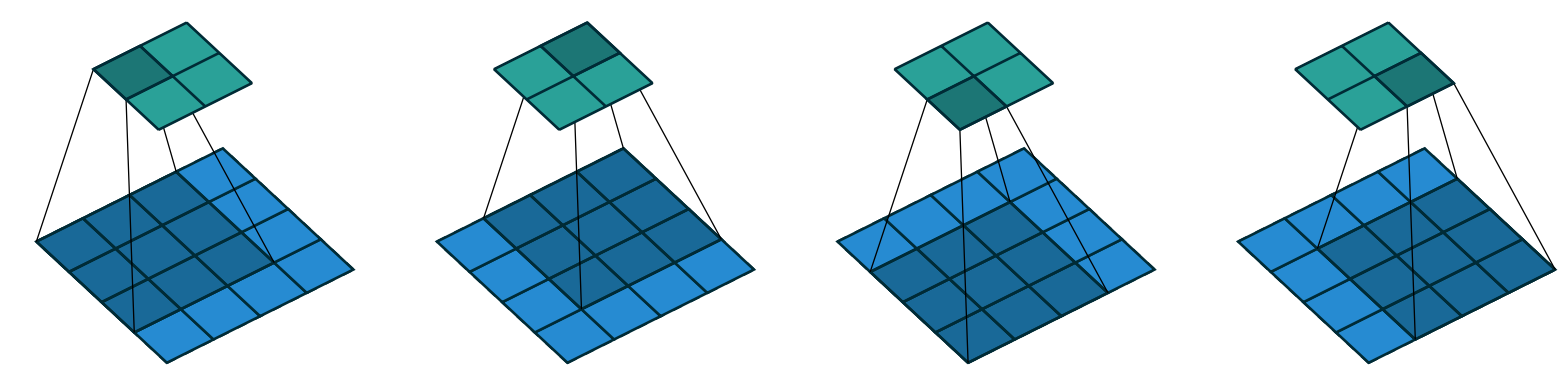
\includegraphics[width=\textwidth]{images/att_00028.png}
    }
    \caption{Depiction of how a convolution computes its outputs. A $4\times 4$ input convolved with a $3\times 3$ kernel produces a $2\times 2$ output. Since no padding is used this constitues a valid convolution. \href{https://fastai.github.io/fastbook2e/images/att_00028.png}{Image Source}}
    \label{fig:convolution}
\end{figure}

The example seen in Figure \ref*{fig:convolution} shows only one channel and a procedure that employs no padding, leaving the output smaller than the input (called a valid convolution). Other than valid convolutions, padding the input by $\lfloor\frac{k}{2}\rfloor$ or $k - 1$, where $k$ is the size of the kernel, leaves us with a \emph{same} (same size as input) or \emph{full} (larger than input) convolution. Additionally, in reality inputs to a layer often have many channels and the layer should be able to produce an arbitrary amount of output channels. In this case there exists a kernel $K_{\text{in}, \text{out}}$ for each combination of input channels $C_\text{in}$ and output channels $C_{\text{out}}$ whose convolution results are then added up for each output channel, so that
$$
    \text{out}_j = \sum_{k=1}^{C_\text{in}} K_{k,j} * \text{input}_k
$$
where $*$ is the convolution operation. There are other approaches to handle multi channel scenarios, but this is the simplest one and the one employed in the thesis.
Another parameter which is often talked about in the context of convolutions is \emph{stride}, which determines by how many units the kernel is moved over the input in each step. The example shown has a stride of 1, but often, a stride of 2 or more may be used when utilising convolutions to downsample inputs.

Using a convolution layer has several advantages over using fully connected layers. First of all is a reduction in \emph{learnable parameters} (see \ref*{sec:training}) which reduces computational resources required and thereby speeds up training. Secondly it introduces the inductive bias that positionally close data points are correlated and relevant to each other to the model, which is reasonable especially in tasks concerning computer vision. 

Imagine having a model that tries to detect circles in an image. It makes sense to assume that features which make up a circle are positionally close to each other. Convolutions are also translationally invariant, which in the same example means that for two identical circles at different locations in the input, the identical output is produced at their corresponing position, which is not the case for fully connected layers, where very different weights might me learned for different positions in the picture if data is insufficiently random.

Many architectures in the computer vision field now purely employ convolutional layers (\emph{fully convolutional neural networks}) or use very few fully connected layers only to compute the final output of the network at the end. 

There are additional constructs that can be used in neural networks, such as \emph{pooling} layers, which also move a kernel over the input like a convolution, but instead take the average or maximum of the covered elements as their output. As such, the pooling layer contains no variable parameters. They are generally used to reduce the dimensions of the feature map to further speed up training time and make the model more stable by promoting invariance to small perturbations in the input.
